% Options for packages loaded elsewhere
\PassOptionsToPackage{unicode}{hyperref}
\PassOptionsToPackage{hyphens}{url}
%
\documentclass[
]{article}
\usepackage{amsmath,amssymb}
\usepackage{lmodern}
\usepackage{ifxetex,ifluatex}
\ifnum 0\ifxetex 1\fi\ifluatex 1\fi=0 % if pdftex
  \usepackage[T1]{fontenc}
  \usepackage[utf8]{inputenc}
  \usepackage{textcomp} % provide euro and other symbols
\else % if luatex or xetex
  \usepackage{unicode-math}
  \defaultfontfeatures{Scale=MatchLowercase}
  \defaultfontfeatures[\rmfamily]{Ligatures=TeX,Scale=1}
\fi
% Use upquote if available, for straight quotes in verbatim environments
\IfFileExists{upquote.sty}{\usepackage{upquote}}{}
\IfFileExists{microtype.sty}{% use microtype if available
  \usepackage[]{microtype}
  \UseMicrotypeSet[protrusion]{basicmath} % disable protrusion for tt fonts
}{}
\makeatletter
\@ifundefined{KOMAClassName}{% if non-KOMA class
  \IfFileExists{parskip.sty}{%
    \usepackage{parskip}
  }{% else
    \setlength{\parindent}{0pt}
    \setlength{\parskip}{6pt plus 2pt minus 1pt}}
}{% if KOMA class
  \KOMAoptions{parskip=half}}
\makeatother
\usepackage{xcolor}
\IfFileExists{xurl.sty}{\usepackage{xurl}}{} % add URL line breaks if available
\IfFileExists{bookmark.sty}{\usepackage{bookmark}}{\usepackage{hyperref}}
\hypersetup{
  pdftitle={Lectura de datos},
  pdfauthor={Maximiliano Cacace},
  hidelinks,
  pdfcreator={LaTeX via pandoc}}
\urlstyle{same} % disable monospaced font for URLs
\usepackage[margin=1in]{geometry}
\usepackage{color}
\usepackage{fancyvrb}
\newcommand{\VerbBar}{|}
\newcommand{\VERB}{\Verb[commandchars=\\\{\}]}
\DefineVerbatimEnvironment{Highlighting}{Verbatim}{commandchars=\\\{\}}
% Add ',fontsize=\small' for more characters per line
\usepackage{framed}
\definecolor{shadecolor}{RGB}{248,248,248}
\newenvironment{Shaded}{\begin{snugshade}}{\end{snugshade}}
\newcommand{\AlertTok}[1]{\textcolor[rgb]{0.94,0.16,0.16}{#1}}
\newcommand{\AnnotationTok}[1]{\textcolor[rgb]{0.56,0.35,0.01}{\textbf{\textit{#1}}}}
\newcommand{\AttributeTok}[1]{\textcolor[rgb]{0.77,0.63,0.00}{#1}}
\newcommand{\BaseNTok}[1]{\textcolor[rgb]{0.00,0.00,0.81}{#1}}
\newcommand{\BuiltInTok}[1]{#1}
\newcommand{\CharTok}[1]{\textcolor[rgb]{0.31,0.60,0.02}{#1}}
\newcommand{\CommentTok}[1]{\textcolor[rgb]{0.56,0.35,0.01}{\textit{#1}}}
\newcommand{\CommentVarTok}[1]{\textcolor[rgb]{0.56,0.35,0.01}{\textbf{\textit{#1}}}}
\newcommand{\ConstantTok}[1]{\textcolor[rgb]{0.00,0.00,0.00}{#1}}
\newcommand{\ControlFlowTok}[1]{\textcolor[rgb]{0.13,0.29,0.53}{\textbf{#1}}}
\newcommand{\DataTypeTok}[1]{\textcolor[rgb]{0.13,0.29,0.53}{#1}}
\newcommand{\DecValTok}[1]{\textcolor[rgb]{0.00,0.00,0.81}{#1}}
\newcommand{\DocumentationTok}[1]{\textcolor[rgb]{0.56,0.35,0.01}{\textbf{\textit{#1}}}}
\newcommand{\ErrorTok}[1]{\textcolor[rgb]{0.64,0.00,0.00}{\textbf{#1}}}
\newcommand{\ExtensionTok}[1]{#1}
\newcommand{\FloatTok}[1]{\textcolor[rgb]{0.00,0.00,0.81}{#1}}
\newcommand{\FunctionTok}[1]{\textcolor[rgb]{0.00,0.00,0.00}{#1}}
\newcommand{\ImportTok}[1]{#1}
\newcommand{\InformationTok}[1]{\textcolor[rgb]{0.56,0.35,0.01}{\textbf{\textit{#1}}}}
\newcommand{\KeywordTok}[1]{\textcolor[rgb]{0.13,0.29,0.53}{\textbf{#1}}}
\newcommand{\NormalTok}[1]{#1}
\newcommand{\OperatorTok}[1]{\textcolor[rgb]{0.81,0.36,0.00}{\textbf{#1}}}
\newcommand{\OtherTok}[1]{\textcolor[rgb]{0.56,0.35,0.01}{#1}}
\newcommand{\PreprocessorTok}[1]{\textcolor[rgb]{0.56,0.35,0.01}{\textit{#1}}}
\newcommand{\RegionMarkerTok}[1]{#1}
\newcommand{\SpecialCharTok}[1]{\textcolor[rgb]{0.00,0.00,0.00}{#1}}
\newcommand{\SpecialStringTok}[1]{\textcolor[rgb]{0.31,0.60,0.02}{#1}}
\newcommand{\StringTok}[1]{\textcolor[rgb]{0.31,0.60,0.02}{#1}}
\newcommand{\VariableTok}[1]{\textcolor[rgb]{0.00,0.00,0.00}{#1}}
\newcommand{\VerbatimStringTok}[1]{\textcolor[rgb]{0.31,0.60,0.02}{#1}}
\newcommand{\WarningTok}[1]{\textcolor[rgb]{0.56,0.35,0.01}{\textbf{\textit{#1}}}}
\usepackage{graphicx}
\makeatletter
\def\maxwidth{\ifdim\Gin@nat@width>\linewidth\linewidth\else\Gin@nat@width\fi}
\def\maxheight{\ifdim\Gin@nat@height>\textheight\textheight\else\Gin@nat@height\fi}
\makeatother
% Scale images if necessary, so that they will not overflow the page
% margins by default, and it is still possible to overwrite the defaults
% using explicit options in \includegraphics[width, height, ...]{}
\setkeys{Gin}{width=\maxwidth,height=\maxheight,keepaspectratio}
% Set default figure placement to htbp
\makeatletter
\def\fps@figure{htbp}
\makeatother
\setlength{\emergencystretch}{3em} % prevent overfull lines
\providecommand{\tightlist}{%
  \setlength{\itemsep}{0pt}\setlength{\parskip}{0pt}}
\setcounter{secnumdepth}{-\maxdimen} % remove section numbering
\ifluatex
  \usepackage{selnolig}  % disable illegal ligatures
\fi

\title{Lectura de datos}
\author{Maximiliano Cacace}
\date{24/5/2021}

\begin{document}
\maketitle

\hypertarget{leer-los-datos}{%
\subsection{Leer los datos}\label{leer-los-datos}}

\begin{Shaded}
\begin{Highlighting}[]
\FunctionTok{library}\NormalTok{(readxl)}
\NormalTok{Becarios\_2020 }\OtherTok{\textless{}{-}} \FunctionTok{read\_excel}\NormalTok{(}\StringTok{"C:/Users/hp/Desktop/TODO/UNSAM/Doctorado Ciencias Humanas/Métodos cuantitativos y análisis de grandes datos/BIG\_DATA\_CACACE/Becarios 2020.xlsx"}\NormalTok{)}
\CommentTok{\#View(Becarios\_2020)}

\NormalTok{Becarios\_2021 }\OtherTok{\textless{}{-}} \FunctionTok{read\_excel}\NormalTok{(}\StringTok{"C:/Users/hp/Desktop/TODO/UNSAM/Doctorado Ciencias Humanas/Métodos cuantitativos y análisis de grandes datos/BIG\_DATA\_CACACE/Becarios 2021.xlsx"}\NormalTok{)}
\end{Highlighting}
\end{Shaded}

\#```\{r CSV\} library(readr) Becarios\_2020 \textless-
read\_delim(``C:/Users/hp/Desktop/TODO/UNSAM/Doctorado Ciencias
Humanas/Métodos cuantitativos y análisis de grandes
datos/BIG\_DATA\_CACACE/Becarios 2020.csv'', ``;'', escape\_double =
FALSE, trim\_ws = TRUE) View(Becarios\_2020)

Becarios\_2021 \textless-
read\_delim(``C:/Users/hp/Desktop/TODO/UNSAM/Doctorado Ciencias
Humanas/Métodos cuantitativos y análisis de grandes
datos/BIG\_DATA\_CACACE/Becarios 2021.csv'', ``;'', escape\_double =
FALSE, trim\_ws = TRUE) View(Becarios\_2021) \#```

\begin{Shaded}
\begin{Highlighting}[]
\FunctionTok{str}\NormalTok{(Becarios\_2020)}
\end{Highlighting}
\end{Shaded}

\begin{verbatim}
## tibble [165 x 30] (S3: tbl_df/tbl/data.frame)
##  $ Edad                                                                   : num [1:165] 22 37 22 22 26 25 25 21 26 22 ...
##  $ Nacionalidad                                                           : chr [1:165] "Argentina" "Argentino" "Argentina" "Argentina" ...
##  $ DNI                                                                    : num [1:165] 40738524 29780468 40676015 40732964 38028913 ...
##  $ Carrera_que_cursa                                                      : chr [1:165] "Ingeniería en Energía" "Ingeniería Espacial" "Ingeniería Electrónica" "Licenciatura en Biotecnología" ...
##  $ Tiempo_de_beca                                                         : chr [1:165] "Este es el primer año" "Este es el primer año" "Este es el primer año" "Este es el primer año" ...
##  $ Costeo_de_estudios                                                     : chr [1:165] "Aportes familiares" "Con dificultad para costear sus estudios" "Aportes familiares" "Con dificultad para costear sus estudios" ...
##  $ Con_quien_vive                                                         : chr [1:165] "Solo" "Familia" "Familia" "Familia" ...
##  $ Por_que_eligio_ la_UNSAM                                               : chr [1:165] "Por el programa de la carrera" "Otro" "Por recomendación" "Por el programa de la carrera" ...
##  $ Educacion_Primaria                                                     : chr [1:165] "Estatal" "Estatal" "Privada" "Estatal" ...
##  $ Educacion_Secundaria                                                   : chr [1:165] "Estatal" "Estatal" "Privada" "Estatal" ...
##  $ Relacion_con_la_carrera                                                : chr [1:165] "SI" "NO" "SI" "SI" ...
##  $ Repitencia_o_abandono_temporal_de_estudios                             : chr [1:165] "No" "No" "No" "No" ...
##  $ Tiempo_transcurrido_desde_el secundario_hasta_ingresar_a_la_universidad: chr [1:165] "Ingresé al año siguiente luego de terminar el secundario." "Más de 5 años" "Ingresé al año siguiente luego de terminar el secundario." "Entre 1 y 5 años" ...
##  $ Que_hizo_en_ese_tiempo                                                 : chr [1:165] "Terminé el secundario, transcurrieron las vacaciones de verano e inmediatamente después empecé el CPU" "Estudie profesorado de matemática y estudie ajedrez" "Receso de verano" "Estudié otras carreras" ...
##  $ Trabajo                                                                : chr [1:165] "No, por decisión propia" "Si" "No, pero se encuentra buscando trabajo" "No, pero se encuentra buscando trabajo" ...
##  $ Que_actividad_desempeña                                                : chr [1:165] NA "Docente particular" NA NA ...
##  $ Horas_semanales_de_trabajo                                             : chr [1:165] NA "Entre 10 y 20 horas" NA NA ...
##  $ Aprobacion_del_CPU                                                     : chr [1:165] "Si" "Si" "Si" "Si" ...
##  $ Año_de_inicio_del_CPU                                                  : num [1:165] 2017 2016 2017 2019 2019 ...
##  $ Cuatrimestre_de_inicio_CPU                                             : chr [1:165] "1er Cuatrimestre" "1er Cuatrimestre" "1er Cuatrimestre" "2do Cuatrimestre" ...
##  $ Alguna_dificultad_en_el_CPU_describir_en_caso_afirmativo               : chr [1:165] "No" "No" "No" "No" ...
##  $ Cuantos_cuatrimestres_le_llevo_aprobar_el_CPU                          : num [1:165] 1 1 1 1 NA 1 2 3 2 1 ...
##  $ Año_de_inicio_de_carrera                                               : num [1:165] 2017 2016 2017 2020 NA ...
##  $ Cuatrimestre_de_inicio_de_carrera                                      : chr [1:165] "2do Cuatrimestre" "1er Cuatrimestre" "2do Cuatrimestre" "1er Cuatrimestre" ...
##  $ Cantidad_de_materias_que cursa                                         : num [1:165] 4 4 3 4 NA 0 4 3 3 3 ...
##  $ Finales_pendientes                                                     : num [1:165] 3 1 0 0 NA 1 0 1 0 5 ...
##  $ Seguimiento_del_plan_de_estudios                                       : chr [1:165] "Parcialmente" "Sí" "Sí" "Sí" ...
##  $ Dificultades_observadas_en_el_seguimiento_del_plan_de_estudios         : chr [1:165] "Acumulación de finales" "Inconvenientes laborales" "No" "Problemas familiares" ...
##  $ Horas_semanales_destinadas_a_estudiar                                  : chr [1:165] "Más de 20 horas" "Entre 10 y 20 horas" "Más de 20 horas" "Entre 10 y 20 horas" ...
##  $ Porque_decidio_estudiar_en_la_Universidad                              : chr [1:165] "Vocación" "Vocación" "Vocación" "Vocación" ...
\end{verbatim}

\hypertarget{cambiar-factor-y-nombre-de-respuesta-de-variable}{%
\subsection{Cambiar factor y nombre de respuesta de
variable}\label{cambiar-factor-y-nombre-de-respuesta-de-variable}}

\begin{Shaded}
\begin{Highlighting}[]
\NormalTok{Becarios\_2020}\SpecialCharTok{$}\NormalTok{Tiempo\_de\_beca }\OtherTok{\textless{}{-}} 
  \FunctionTok{factor}\NormalTok{(}\FunctionTok{as.character}\NormalTok{(Becarios\_2020}\SpecialCharTok{$}\NormalTok{Tiempo\_de\_beca), }
         \AttributeTok{labels =} \FunctionTok{c}\NormalTok{(}\StringTok{"Este es el primer año"} \OtherTok{=} \StringTok{"0.5"}\NormalTok{,}
                    \StringTok{"1 año"} \OtherTok{=} \StringTok{"1"}\NormalTok{,}
                    \StringTok{"2 años"} \OtherTok{=} \StringTok{"2"}\NormalTok{,}
                    \StringTok{"3 años"} \OtherTok{=} \StringTok{"3"}\NormalTok{,}
                    \StringTok{"4 años"} \OtherTok{=} \StringTok{"4"}\NormalTok{)}
\NormalTok{  )}

\NormalTok{Becarios\_2020}\SpecialCharTok{$}\NormalTok{Tiempo\_de\_beca }\OtherTok{\textless{}{-}} 
  \FunctionTok{as.numeric}\NormalTok{(Becarios\_2020}\SpecialCharTok{$}\NormalTok{Tiempo\_de\_beca)}
\end{Highlighting}
\end{Shaded}

\begin{Shaded}
\begin{Highlighting}[]
\NormalTok{Becarios\_2020}\SpecialCharTok{$}\NormalTok{Tiempo\_de\_beca }\SpecialCharTok{\%\textgreater{}\%}
  \FunctionTok{class}\NormalTok{()}
\end{Highlighting}
\end{Shaded}

\begin{verbatim}
## [1] "numeric"
\end{verbatim}

\begin{Shaded}
\begin{Highlighting}[]
\FunctionTok{table}\NormalTok{(Becarios\_2020}\SpecialCharTok{$}\NormalTok{Tiempo\_de\_beca)}
\end{Highlighting}
\end{Shaded}

\begin{verbatim}
## 
##  1  2  3  4  5 
## 31 17 14  6 97
\end{verbatim}

\begin{Shaded}
\begin{Highlighting}[]
\NormalTok{Becarios\_2020}\SpecialCharTok{$}\NormalTok{Cuatrimestre\_de\_inicio\_CPU }\OtherTok{\textless{}{-}} 
  \FunctionTok{factor}\NormalTok{(}\FunctionTok{as.character}\NormalTok{(Becarios\_2020}\SpecialCharTok{$}\NormalTok{Cuatrimestre\_de\_inicio\_CPU), }
         \AttributeTok{labels =} \FunctionTok{c}\NormalTok{(}\StringTok{"1er Cuatrimestre"} \OtherTok{=} \StringTok{"1"}\NormalTok{,}
                    \StringTok{"2do Cuatrimestre"} \OtherTok{=} \StringTok{"2"}\NormalTok{)}
\NormalTok{  )}

\NormalTok{Becarios\_2020}\SpecialCharTok{$}\NormalTok{Cuatrimestre\_de\_inicio\_CPU }\OtherTok{\textless{}{-}} 
  \FunctionTok{factor}\NormalTok{(}\FunctionTok{as.numeric}\NormalTok{(Becarios\_2020}\SpecialCharTok{$}\NormalTok{Cuatrimestre\_de\_inicio\_CPU), }
         \AttributeTok{labels =} \FunctionTok{c}\NormalTok{(}\StringTok{"1"} \OtherTok{=} \StringTok{"1"}\NormalTok{,}
                    \StringTok{"2"} \OtherTok{=} \StringTok{"2"}\NormalTok{)}
\NormalTok{  )}
\NormalTok{Becarios\_2020}\SpecialCharTok{$}\NormalTok{Cuatrimestre\_de\_inicio\_CPU }\SpecialCharTok{\%\textgreater{}\%}
  \FunctionTok{class}\NormalTok{()}
\end{Highlighting}
\end{Shaded}

\begin{verbatim}
## [1] "factor"
\end{verbatim}

\begin{Shaded}
\begin{Highlighting}[]
\FunctionTok{table}\NormalTok{(Becarios\_2020}\SpecialCharTok{$}\NormalTok{Cuatrimestre\_de\_inicio\_CPU)}
\end{Highlighting}
\end{Shaded}

\begin{verbatim}
## 
##   1   2 
## 132  33
\end{verbatim}

\begin{Shaded}
\begin{Highlighting}[]
\NormalTok{Becarios\_2020}\SpecialCharTok{$}\NormalTok{Cuatrimestre\_de\_inicio\_CPU }\SpecialCharTok{\%\textgreater{}\%}
  \FunctionTok{class}\NormalTok{()}
\end{Highlighting}
\end{Shaded}

\begin{verbatim}
## [1] "factor"
\end{verbatim}

\begin{Shaded}
\begin{Highlighting}[]
\FunctionTok{table}\NormalTok{(Becarios\_2020}\SpecialCharTok{$}\NormalTok{Cuatrimestre\_de\_inicio\_CPU)}
\end{Highlighting}
\end{Shaded}

\begin{verbatim}
## 
##   1   2 
## 132  33
\end{verbatim}

\begin{Shaded}
\begin{Highlighting}[]
\FunctionTok{nrow}\NormalTok{(Becarios\_2020)}
\end{Highlighting}
\end{Shaded}

\begin{verbatim}
## [1] 165
\end{verbatim}

\begin{Shaded}
\begin{Highlighting}[]
\FunctionTok{ncol}\NormalTok{(Becarios\_2020)}
\end{Highlighting}
\end{Shaded}

\begin{verbatim}
## [1] 30
\end{verbatim}

\begin{Shaded}
\begin{Highlighting}[]
\FunctionTok{nrow}\NormalTok{(Becarios\_2021)}
\end{Highlighting}
\end{Shaded}

\begin{verbatim}
## [1] 151
\end{verbatim}

\begin{Shaded}
\begin{Highlighting}[]
\FunctionTok{ncol}\NormalTok{(Becarios\_2021)}
\end{Highlighting}
\end{Shaded}

\begin{verbatim}
## [1] 30
\end{verbatim}

\begin{Shaded}
\begin{Highlighting}[]
\CommentTok{\#Ratio = 8}
\CommentTok{\#Nominal = 22}

\NormalTok{Becarios\_2020}\SpecialCharTok{$}\NormalTok{Edad }\SpecialCharTok{\%\textgreater{}\%} \CommentTok{\#Ratio}
  \FunctionTok{class}\NormalTok{()}
\end{Highlighting}
\end{Shaded}

\begin{verbatim}
## [1] "numeric"
\end{verbatim}

\begin{Shaded}
\begin{Highlighting}[]
\NormalTok{Becarios\_2020}\SpecialCharTok{$}\NormalTok{Nacionalidad }\SpecialCharTok{\%\textgreater{}\%} \CommentTok{\#Nominal}
  \FunctionTok{class}\NormalTok{()}
\end{Highlighting}
\end{Shaded}

\begin{verbatim}
## [1] "character"
\end{verbatim}

\begin{Shaded}
\begin{Highlighting}[]
\NormalTok{Becarios\_2020}\SpecialCharTok{$}\NormalTok{DNI }\SpecialCharTok{\%\textgreater{}\%} \CommentTok{\#Nominal}
  \FunctionTok{class}\NormalTok{()}
\end{Highlighting}
\end{Shaded}

\begin{verbatim}
## [1] "numeric"
\end{verbatim}

\begin{Shaded}
\begin{Highlighting}[]
\NormalTok{Becarios\_2020}\SpecialCharTok{$}\NormalTok{Carrera\_que\_cursa }\SpecialCharTok{\%\textgreater{}\%} \CommentTok{\#Nominal}
  \FunctionTok{class}\NormalTok{()}
\end{Highlighting}
\end{Shaded}

\begin{verbatim}
## [1] "character"
\end{verbatim}

\begin{Shaded}
\begin{Highlighting}[]
\NormalTok{Becarios\_2020}\SpecialCharTok{$}\NormalTok{Tiempo\_de\_beca }\SpecialCharTok{\%\textgreater{}\%} \CommentTok{\#Ratio}
  \FunctionTok{class}\NormalTok{()}
\end{Highlighting}
\end{Shaded}

\begin{verbatim}
## [1] "numeric"
\end{verbatim}

\begin{Shaded}
\begin{Highlighting}[]
\NormalTok{Becarios\_2020}\SpecialCharTok{$}\NormalTok{Costeo\_de\_estudios }\SpecialCharTok{\%\textgreater{}\%} \CommentTok{\#Nominal}
  \FunctionTok{class}\NormalTok{()}
\end{Highlighting}
\end{Shaded}

\begin{verbatim}
## [1] "character"
\end{verbatim}

\begin{Shaded}
\begin{Highlighting}[]
\NormalTok{Becarios\_2020}\SpecialCharTok{$}\NormalTok{Con\_quien\_vive }\SpecialCharTok{\%\textgreater{}\%} \CommentTok{\#Nominal}
  \FunctionTok{class}\NormalTok{()}
\end{Highlighting}
\end{Shaded}

\begin{verbatim}
## [1] "character"
\end{verbatim}

\begin{Shaded}
\begin{Highlighting}[]
\NormalTok{Becarios\_2020}\SpecialCharTok{$}\StringTok{\textasciigrave{}}\AttributeTok{Por\_que\_eligio\_ la\_UNSAM}\StringTok{\textasciigrave{}} \SpecialCharTok{\%\textgreater{}\%} \CommentTok{\#Nominal}
  \FunctionTok{class}\NormalTok{()}
\end{Highlighting}
\end{Shaded}

\begin{verbatim}
## [1] "character"
\end{verbatim}

\begin{Shaded}
\begin{Highlighting}[]
\NormalTok{Becarios\_2020}\SpecialCharTok{$}\NormalTok{Educacion\_Primaria }\SpecialCharTok{\%\textgreater{}\%} \CommentTok{\#Nominal}
  \FunctionTok{class}\NormalTok{()}
\end{Highlighting}
\end{Shaded}

\begin{verbatim}
## [1] "character"
\end{verbatim}

\begin{Shaded}
\begin{Highlighting}[]
\NormalTok{Becarios\_2020}\SpecialCharTok{$}\NormalTok{Educacion\_Secundaria }\SpecialCharTok{\%\textgreater{}\%} \CommentTok{\#Nominal}
  \FunctionTok{class}\NormalTok{()}
\end{Highlighting}
\end{Shaded}

\begin{verbatim}
## [1] "character"
\end{verbatim}

\begin{Shaded}
\begin{Highlighting}[]
\NormalTok{Becarios\_2020}\SpecialCharTok{$}\NormalTok{Relacion\_con\_la\_carrera }\SpecialCharTok{\%\textgreater{}\%} \CommentTok{\#Nominal}
  \FunctionTok{class}\NormalTok{()}
\end{Highlighting}
\end{Shaded}

\begin{verbatim}
## [1] "character"
\end{verbatim}

\begin{Shaded}
\begin{Highlighting}[]
\NormalTok{Becarios\_2020}\SpecialCharTok{$}\NormalTok{Repitencia\_o\_abandono\_temporal\_de\_estudios }\SpecialCharTok{\%\textgreater{}\%} \CommentTok{\#Nominal}
  \FunctionTok{class}\NormalTok{()}
\end{Highlighting}
\end{Shaded}

\begin{verbatim}
## [1] "character"
\end{verbatim}

\begin{Shaded}
\begin{Highlighting}[]
\NormalTok{Becarios\_2020}\SpecialCharTok{$}\StringTok{\textasciigrave{}}\AttributeTok{Tiempo\_transcurrido\_desde\_el secundario\_hasta\_ingresar\_a\_la\_universidad}\StringTok{\textasciigrave{}} \SpecialCharTok{\%\textgreater{}\%} \CommentTok{\#Ratio}
  \FunctionTok{class}\NormalTok{()}
\end{Highlighting}
\end{Shaded}

\begin{verbatim}
## [1] "character"
\end{verbatim}

\begin{Shaded}
\begin{Highlighting}[]
\NormalTok{Becarios\_2020}\SpecialCharTok{$}\NormalTok{Que\_hizo\_en\_ese\_tiempo }\SpecialCharTok{\%\textgreater{}\%} \CommentTok{\#Nominal}
  \FunctionTok{class}\NormalTok{()}
\end{Highlighting}
\end{Shaded}

\begin{verbatim}
## [1] "character"
\end{verbatim}

\begin{Shaded}
\begin{Highlighting}[]
\NormalTok{Becarios\_2020}\SpecialCharTok{$}\NormalTok{Trabajo }\SpecialCharTok{\%\textgreater{}\%} \CommentTok{\#Nominal}
  \FunctionTok{class}\NormalTok{()}
\end{Highlighting}
\end{Shaded}

\begin{verbatim}
## [1] "character"
\end{verbatim}

\begin{Shaded}
\begin{Highlighting}[]
\NormalTok{Becarios\_2020}\SpecialCharTok{$}\NormalTok{Que\_actividad\_desempeña }\SpecialCharTok{\%\textgreater{}\%} \CommentTok{\#Nominal}
  \FunctionTok{class}\NormalTok{()}
\end{Highlighting}
\end{Shaded}

\begin{verbatim}
## [1] "character"
\end{verbatim}

\begin{Shaded}
\begin{Highlighting}[]
\NormalTok{Becarios\_2020}\SpecialCharTok{$}\NormalTok{Horas\_semanales\_de\_trabajo }\SpecialCharTok{\%\textgreater{}\%} \CommentTok{\#Ratio}
  \FunctionTok{class}\NormalTok{()}
\end{Highlighting}
\end{Shaded}

\begin{verbatim}
## [1] "character"
\end{verbatim}

\begin{Shaded}
\begin{Highlighting}[]
\NormalTok{Becarios\_2020}\SpecialCharTok{$}\NormalTok{Aprobacion\_del\_CPU }\SpecialCharTok{\%\textgreater{}\%} \CommentTok{\#Nominal}
  \FunctionTok{class}\NormalTok{()}
\end{Highlighting}
\end{Shaded}

\begin{verbatim}
## [1] "character"
\end{verbatim}

\begin{Shaded}
\begin{Highlighting}[]
\NormalTok{Becarios\_2020}\SpecialCharTok{$}\NormalTok{Año\_de\_inicio\_del\_CPU }\SpecialCharTok{\%\textgreater{}\%} \CommentTok{\#Nominal}
  \FunctionTok{class}\NormalTok{()}
\end{Highlighting}
\end{Shaded}

\begin{verbatim}
## [1] "numeric"
\end{verbatim}

\begin{Shaded}
\begin{Highlighting}[]
\NormalTok{Becarios\_2020}\SpecialCharTok{$}\NormalTok{Cuatrimestre\_de\_inicio\_CPU }\SpecialCharTok{\%\textgreater{}\%} \CommentTok{\#Nominal}
  \FunctionTok{class}\NormalTok{()}
\end{Highlighting}
\end{Shaded}

\begin{verbatim}
## [1] "factor"
\end{verbatim}

\begin{Shaded}
\begin{Highlighting}[]
\NormalTok{Becarios\_2020}\SpecialCharTok{$}\NormalTok{Alguna\_dificultad\_en\_el\_CPU\_describir\_en\_caso\_afirmativo }\SpecialCharTok{\%\textgreater{}\%} \CommentTok{\#Nominal}
  \FunctionTok{class}\NormalTok{()}
\end{Highlighting}
\end{Shaded}

\begin{verbatim}
## [1] "character"
\end{verbatim}

\begin{Shaded}
\begin{Highlighting}[]
\NormalTok{Becarios\_2020}\SpecialCharTok{$}\NormalTok{Cuantos\_cuatrimestres\_le\_llevo\_aprobar\_el\_CPU }\SpecialCharTok{\%\textgreater{}\%} \CommentTok{\#Ratio}
  \FunctionTok{class}\NormalTok{()}
\end{Highlighting}
\end{Shaded}

\begin{verbatim}
## [1] "numeric"
\end{verbatim}

\begin{Shaded}
\begin{Highlighting}[]
\NormalTok{Becarios\_2020}\SpecialCharTok{$}\NormalTok{Año\_de\_inicio\_de\_carrera }\SpecialCharTok{\%\textgreater{}\%} \CommentTok{\#Nominal}
  \FunctionTok{class}\NormalTok{()}
\end{Highlighting}
\end{Shaded}

\begin{verbatim}
## [1] "numeric"
\end{verbatim}

\begin{Shaded}
\begin{Highlighting}[]
\NormalTok{Becarios\_2020}\SpecialCharTok{$}\NormalTok{Cuatrimestre\_de\_inicio\_de\_carrera }\SpecialCharTok{\%\textgreater{}\%} \CommentTok{\#Nominal}
  \FunctionTok{class}\NormalTok{()}
\end{Highlighting}
\end{Shaded}

\begin{verbatim}
## [1] "character"
\end{verbatim}

\begin{Shaded}
\begin{Highlighting}[]
\NormalTok{Becarios\_2020}\SpecialCharTok{$}\StringTok{\textasciigrave{}}\AttributeTok{Cantidad\_de\_materias\_que cursa}\StringTok{\textasciigrave{}} \SpecialCharTok{\%\textgreater{}\%} \CommentTok{\#Ratio}
  \FunctionTok{class}\NormalTok{()}
\end{Highlighting}
\end{Shaded}

\begin{verbatim}
## [1] "numeric"
\end{verbatim}

\begin{Shaded}
\begin{Highlighting}[]
\NormalTok{Becarios\_2020}\SpecialCharTok{$}\NormalTok{Finales\_pendientes }\SpecialCharTok{\%\textgreater{}\%} \CommentTok{\#Ratio}
  \FunctionTok{class}\NormalTok{()}
\end{Highlighting}
\end{Shaded}

\begin{verbatim}
## [1] "numeric"
\end{verbatim}

\begin{Shaded}
\begin{Highlighting}[]
\NormalTok{Becarios\_2020}\SpecialCharTok{$}\NormalTok{Seguimiento\_del\_plan\_de\_estudios }\SpecialCharTok{\%\textgreater{}\%} \CommentTok{\#Nominal}
  \FunctionTok{class}\NormalTok{()}
\end{Highlighting}
\end{Shaded}

\begin{verbatim}
## [1] "character"
\end{verbatim}

\begin{Shaded}
\begin{Highlighting}[]
\NormalTok{Becarios\_2020}\SpecialCharTok{$}\NormalTok{Dificultades\_observadas\_en\_el\_seguimiento\_del\_plan\_de\_estudios }\SpecialCharTok{\%\textgreater{}\%} \CommentTok{\#Nominal}
  \FunctionTok{class}\NormalTok{()}
\end{Highlighting}
\end{Shaded}

\begin{verbatim}
## [1] "character"
\end{verbatim}

\begin{Shaded}
\begin{Highlighting}[]
\NormalTok{Becarios\_2020}\SpecialCharTok{$}\NormalTok{Horas\_semanales\_destinadas\_a\_estudiar }\SpecialCharTok{\%\textgreater{}\%} \CommentTok{\#Ratio}
  \FunctionTok{class}\NormalTok{()}
\end{Highlighting}
\end{Shaded}

\begin{verbatim}
## [1] "character"
\end{verbatim}

\begin{Shaded}
\begin{Highlighting}[]
\NormalTok{Becarios\_2020}\SpecialCharTok{$}\NormalTok{Porque\_decidio\_estudiar\_en\_la\_Universidad }\SpecialCharTok{\%\textgreater{}\%} \CommentTok{\#Nominal}
  \FunctionTok{class}\NormalTok{()}
\end{Highlighting}
\end{Shaded}

\begin{verbatim}
## [1] "character"
\end{verbatim}

\begin{Shaded}
\begin{Highlighting}[]
\NormalTok{Becarios\_2020}\SpecialCharTok{$}\NormalTok{Edad}
\end{Highlighting}
\end{Shaded}

\begin{verbatim}
##   [1] 22 37 22 22 26 25 25 21 26 22 20 26 20 36 18 20 17 19 26 34 21 22 19 25 25
##  [26] 18 22 59 32 25 22 20 26 21 29 22 20 27 33 23 22 19 22 45 28 32 33 25 60 30
##  [51] 27 23 24 24 18 18 24 26 48 27 25 19 20 25 25 29 22 25 18 26 29 32 22 28 21
##  [76] 23 22 22 19 22 20 20 23 24 42 24 18 25 29 25 19 33 22 43 27 23 26 35 24 20
## [101] 32 20 22 21 20 20 21 25 23 22 22 19 30 20 17 25 37 19 20 20 21 23 37 18 28
## [126] 31 23 20 19 19 20 32 23 20 26 22 25 27 26 21 27 21 25 23 23 35 24 20 20 22
## [151] 20 33 34 36 19 19 25 23 26 20 25 18 19 19 24
\end{verbatim}

\begin{Shaded}
\begin{Highlighting}[]
\NormalTok{Becarios\_2021}\SpecialCharTok{$}\NormalTok{Edad}
\end{Highlighting}
\end{Shaded}

\begin{verbatim}
##   [1] 26 23 22 22 26 55 21 27 18 21 37 21 20 44 27 24 24 23 29 26 36 23 21 48 28
##  [26] 23 28 23 17 40 19 42 46 29 33 34 26 19 30 36 31 20 24 25 25 20 49 28 18 30
##  [51] 23 20 26 30 26 23 19 21 27 30 32 23 25 38 22 23 20 26 26 21 20 21 25 27 43
##  [76] 26 20 22 26 34 45 24 27 33 36 26 25 21 21 23 21 22 26 42 24 19 23 35 31 22
## [101] 23 25 38 20 23 28 21 22 25 38 19 25 22 34 23 19 24 51 21 26 41 23 33 22 27
## [126] 39 23 18 28 22 20 22 26 23 36 21 25 25 21 23 20 23 19 29 34 20 21 23 22 24
## [151] 29
\end{verbatim}

\begin{Shaded}
\begin{Highlighting}[]
\FunctionTok{table}\NormalTok{(Becarios\_2020}\SpecialCharTok{$}\NormalTok{Edad)}
\end{Highlighting}
\end{Shaded}

\begin{verbatim}
## 
## 17 18 19 20 21 22 23 24 25 26 27 28 29 30 31 32 33 34 35 36 37 42 43 45 48 59 
##  2  8 14 22  9 21 12  8 18 11  6  3  4  2  1  5  4  2  2  2  3  1  1  1  1  1 
## 60 
##  1
\end{verbatim}

\begin{Shaded}
\begin{Highlighting}[]
\FunctionTok{table}\NormalTok{(Becarios\_2021}\SpecialCharTok{$}\NormalTok{Edad)}
\end{Highlighting}
\end{Shaded}

\begin{verbatim}
## 
## 17 18 19 20 21 22 23 24 25 26 27 28 29 30 31 32 33 34 35 36 37 38 39 40 41 42 
##  1  3  7 11 15 12 20  7 10 14  6  5  4  4  2  1  3  4  1  4  1  3  1  1  1  2 
## 43 44 45 46 48 49 51 55 
##  1  1  1  1  1  1  1  1
\end{verbatim}

\begin{Shaded}
\begin{Highlighting}[]
\FunctionTok{table}\NormalTok{(Becarios\_2020}\SpecialCharTok{$}\NormalTok{Carrera\_que\_cursa)}
\end{Highlighting}
\end{Shaded}

\begin{verbatim}
## 
##                    Ingeniería Ambiental                    Ingeniería Biomédica 
##                                      20                                      12 
##                  Ingeniería Electrónica                   Ingeniería en Energía 
##                                      10                                      10 
##        Ingeniería en Telecomunicaciones                     Ingeniería Espacial 
##                                       4                                       3 
##                   Ingeniería Industrial           Licenciatura en Biotecnología 
##                                       8                                      40 
##           Licenciatura en Física Médica Tecnicatura en Diagnóstico por Imágenes 
##                                       4                                      38 
##          Tecnicatura en Electromedicina Tecnicatura en Programación Informática 
##                                       2                                      12 
##       Tecnicatura en Redes Informáticas 
##                                       2
\end{verbatim}

\begin{Shaded}
\begin{Highlighting}[]
\NormalTok{Becarios\_2020 }\SpecialCharTok{\%\textgreater{}\%} 
   \FunctionTok{group\_by}\NormalTok{(Costeo\_de\_estudios) }\SpecialCharTok{\%\textgreater{}\%} 
   \FunctionTok{summarize}\NormalTok{(}
     \FunctionTok{mean}\NormalTok{(Edad),}
     \FunctionTok{median}\NormalTok{(Edad)}
\NormalTok{   )}
\end{Highlighting}
\end{Shaded}

\begin{verbatim}
## # A tibble: 5 x 3
##   Costeo_de_estudios                       `mean(Edad)` `median(Edad)`
##   <chr>                                           <dbl>          <dbl>
## 1 Aportes familiares                               22.4           22  
## 2 Beca                                             23.8           22  
## 3 Con dificultad para costear sus estudios         26.9           25.5
## 4 Plan social                                      60             60  
## 5 Trabajo                                          27.4           24.5
\end{verbatim}

\begin{Shaded}
\begin{Highlighting}[]
\FunctionTok{mean}\NormalTok{(Becarios\_2020}\SpecialCharTok{$}\NormalTok{Edad) }\OtherTok{{-}\textgreater{}}\NormalTok{ promedio\_Edad2020}
\NormalTok{promedio\_Edad2020}
\end{Highlighting}
\end{Shaded}

\begin{verbatim}
## [1] 24.86061
\end{verbatim}

\begin{Shaded}
\begin{Highlighting}[]
\FunctionTok{mean}\NormalTok{(Becarios\_2021}\SpecialCharTok{$}\NormalTok{Edad) }\OtherTok{{-}\textgreater{}}\NormalTok{ promedio\_Edad2021}
\NormalTok{promedio\_Edad2021}
\end{Highlighting}
\end{Shaded}

\begin{verbatim}
## [1] 26.66887
\end{verbatim}

\begin{Shaded}
\begin{Highlighting}[]
\FunctionTok{median}\NormalTok{(Becarios\_2020}\SpecialCharTok{$}\NormalTok{Edad) }\OtherTok{{-}\textgreater{}}\NormalTok{ median\_Edad2020 }
\NormalTok{median\_Edad2020}
\end{Highlighting}
\end{Shaded}

\begin{verbatim}
## [1] 23
\end{verbatim}

\begin{Shaded}
\begin{Highlighting}[]
\FunctionTok{median}\NormalTok{(Becarios\_2021}\SpecialCharTok{$}\NormalTok{Edad) }\OtherTok{{-}\textgreater{}}\NormalTok{ median\_Edad2021}
\NormalTok{median\_Edad2021}
\end{Highlighting}
\end{Shaded}

\begin{verbatim}
## [1] 24
\end{verbatim}

\begin{Shaded}
\begin{Highlighting}[]
\FunctionTok{range}\NormalTok{(Becarios\_2020}\SpecialCharTok{$}\NormalTok{Edad) }\CommentTok{\#Rango o Amplitud de la variable (valor máx. y min.)}
\end{Highlighting}
\end{Shaded}

\begin{verbatim}
## [1] 17 60
\end{verbatim}

\begin{Shaded}
\begin{Highlighting}[]
\FunctionTok{quantile}\NormalTok{(Becarios\_2020}\SpecialCharTok{$}\NormalTok{Edad) }\CommentTok{\#Cuantiles, deciles y percentiles (se dividen las obs. en 4 partes iguales = 5 valores)}
\end{Highlighting}
\end{Shaded}

\begin{verbatim}
##   0%  25%  50%  75% 100% 
##   17   20   23   26   60
\end{verbatim}

\begin{Shaded}
\begin{Highlighting}[]
\FunctionTok{IQR}\NormalTok{(Becarios\_2020}\SpecialCharTok{$}\NormalTok{Edad) }\CommentTok{\#Rango intercuartil (diferencia entre el tercer y el primer cuartil de una distribución)}
\end{Highlighting}
\end{Shaded}

\begin{verbatim}
## [1] 6
\end{verbatim}

\begin{Shaded}
\begin{Highlighting}[]
\FunctionTok{var}\NormalTok{(Becarios\_2020}\SpecialCharTok{$}\NormalTok{Edad) }\CommentTok{\#Varianza}
\end{Highlighting}
\end{Shaded}

\begin{verbatim}
## [1] 46.53533
\end{verbatim}

\begin{Shaded}
\begin{Highlighting}[]
\FunctionTok{sd}\NormalTok{(Becarios\_2020}\SpecialCharTok{$}\NormalTok{Edad) }\CommentTok{\#Desviación Estándar}
\end{Highlighting}
\end{Shaded}

\begin{verbatim}
## [1] 6.821681
\end{verbatim}

\begin{Shaded}
\begin{Highlighting}[]
\FunctionTok{mad}\NormalTok{(Becarios\_2020}\SpecialCharTok{$}\NormalTok{Edad) }\CommentTok{\#Desviación Mediana Absoluta}
\end{Highlighting}
\end{Shaded}

\begin{verbatim}
## [1] 4.4478
\end{verbatim}

\begin{Shaded}
\begin{Highlighting}[]
\FunctionTok{summary}\NormalTok{(Becarios\_2020}\SpecialCharTok{$}\NormalTok{Edad)}
\end{Highlighting}
\end{Shaded}

\begin{verbatim}
##    Min. 1st Qu.  Median    Mean 3rd Qu.    Max. 
##   17.00   20.00   23.00   24.86   26.00   60.00
\end{verbatim}

\begin{Shaded}
\begin{Highlighting}[]
\FunctionTok{pnorm}\NormalTok{(Becarios\_2020}\SpecialCharTok{$}\NormalTok{Edad)}
\end{Highlighting}
\end{Shaded}

\begin{verbatim}
##   [1] 1 1 1 1 1 1 1 1 1 1 1 1 1 1 1 1 1 1 1 1 1 1 1 1 1 1 1 1 1 1 1 1 1 1 1 1 1
##  [38] 1 1 1 1 1 1 1 1 1 1 1 1 1 1 1 1 1 1 1 1 1 1 1 1 1 1 1 1 1 1 1 1 1 1 1 1 1
##  [75] 1 1 1 1 1 1 1 1 1 1 1 1 1 1 1 1 1 1 1 1 1 1 1 1 1 1 1 1 1 1 1 1 1 1 1 1 1
## [112] 1 1 1 1 1 1 1 1 1 1 1 1 1 1 1 1 1 1 1 1 1 1 1 1 1 1 1 1 1 1 1 1 1 1 1 1 1
## [149] 1 1 1 1 1 1 1 1 1 1 1 1 1 1 1 1 1
\end{verbatim}

\begin{Shaded}
\begin{Highlighting}[]
\FunctionTok{order}\NormalTok{(Becarios\_2020}\SpecialCharTok{$}\NormalTok{Edad, }\AttributeTok{decreasing=}\ConstantTok{FALSE}\NormalTok{)}
\end{Highlighting}
\end{Shaded}

\begin{verbatim}
##   [1]  17 115  15  26  55  56  69  87 124 162  18  23  42  62  79  91 112 118
##  [19] 129 130 155 156 163 164  11  13  16  32  37  63  81  82 100 102 105 106
##  [37] 114 119 120 128 131 134 148 149 151 160   8  21  34  75 104 107 121 140
##  [55] 142   1   3   4  10  22  27  31  36  41  43  67  73  77  78  80  93 103
##  [73] 110 111 136 150  40  52  76  83  96 109 122 127 133 144 145 158  53  54
##  [91]  57  84  86  99 147 165   6   7  24  25  30  48  61  64  65  68  88  90
## [109] 108 116 137 143 157 161   5   9  12  19  33  58  70  97 135 139 159  38
## [127]  51  60  95 138 141  45  74 125  35  66  71  89  50 113 126  29  46  72
## [145] 101 132  39  47  92 152  20 153  98 146  14 154   2 117 123  85  94  44
## [163]  59  28  49
\end{verbatim}

\hypertarget{tests}{%
\subsection{Tests}\label{tests}}

\begin{Shaded}
\begin{Highlighting}[]
\FunctionTok{shapiro.test}\NormalTok{(Becarios\_2020}\SpecialCharTok{$}\NormalTok{Edad)}
\end{Highlighting}
\end{Shaded}

\begin{verbatim}
## 
##  Shapiro-Wilk normality test
## 
## data:  Becarios_2020$Edad
## W = 0.78464, p-value = 2.625e-14
\end{verbatim}

\begin{Shaded}
\begin{Highlighting}[]
\FunctionTok{t.test}\NormalTok{(Becarios\_2020}\SpecialCharTok{$}\NormalTok{Edad, Becarios\_2021}\SpecialCharTok{$}\NormalTok{Edad)}
\end{Highlighting}
\end{Shaded}

\begin{verbatim}
## 
##  Welch Two Sample t-test
## 
## data:  Becarios_2020$Edad and Becarios_2021$Edad
## t = -2.243, df = 304.47, p-value = 0.02562
## alternative hypothesis: true difference in means is not equal to 0
## 95 percent confidence interval:
##  -3.3946927 -0.2218436
## sample estimates:
## mean of x mean of y 
##  24.86061  26.66887
\end{verbatim}

\#\#Visualización de datos

\begin{Shaded}
\begin{Highlighting}[]
\FunctionTok{hist}\NormalTok{(Becarios\_2020}\SpecialCharTok{$}\NormalTok{Edad)}
\end{Highlighting}
\end{Shaded}

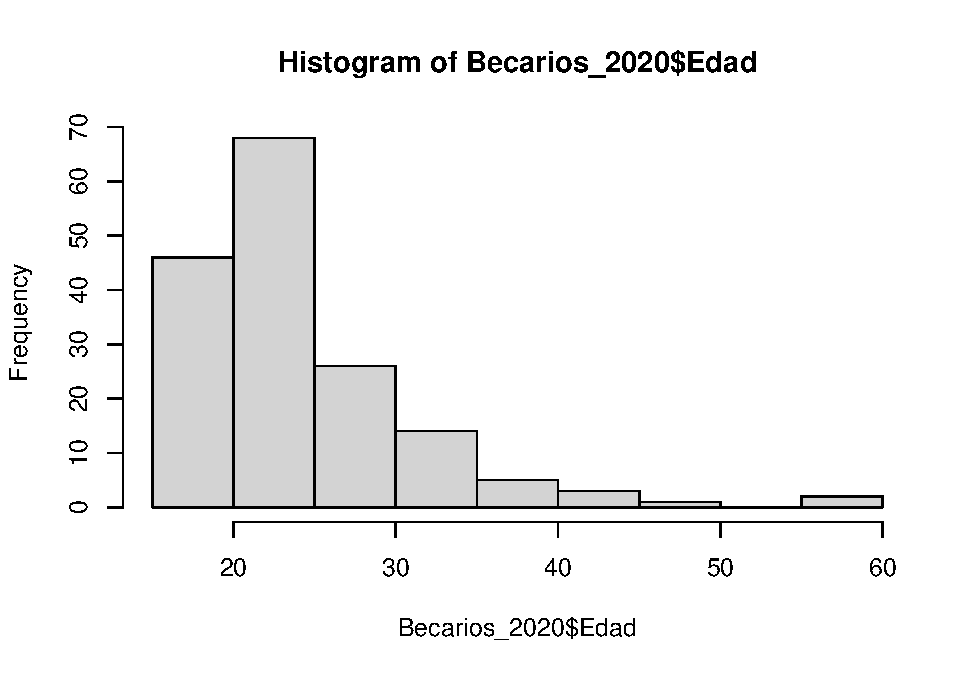
\includegraphics{1-Lectura-de-datos_files/figure-latex/Histograma-1.pdf}

\begin{Shaded}
\begin{Highlighting}[]
\FunctionTok{hist}\NormalTok{(Becarios\_2021}\SpecialCharTok{$}\NormalTok{Edad)}
\end{Highlighting}
\end{Shaded}

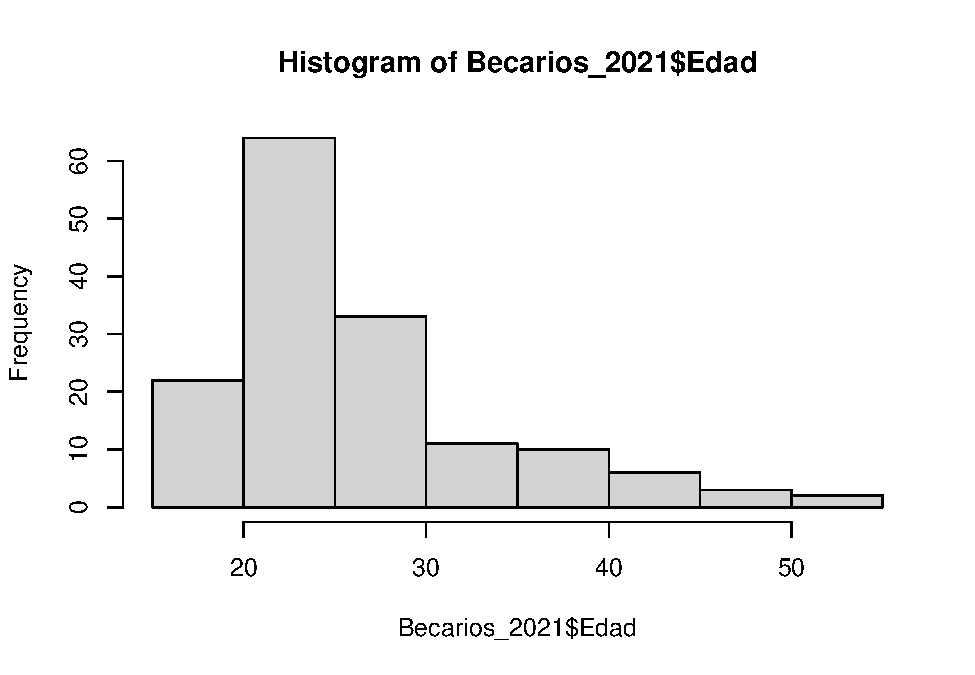
\includegraphics{1-Lectura-de-datos_files/figure-latex/Histograma-2.pdf}

\begin{Shaded}
\begin{Highlighting}[]
\CommentTok{\#polygon(Becarios\_2020$Edad)}
\end{Highlighting}
\end{Shaded}

\begin{Shaded}
\begin{Highlighting}[]
\FunctionTok{boxplot}\NormalTok{(Becarios\_2020}\SpecialCharTok{$}\NormalTok{Edad) }\CommentTok{\#visualización de la dispersión}
\end{Highlighting}
\end{Shaded}

\includegraphics{1-Lectura-de-datos_files/figure-latex/unnamed-chunk-3-1.pdf}

\begin{Shaded}
\begin{Highlighting}[]
\FunctionTok{library}\NormalTok{(ggplot2)}
\NormalTok{Becarios\_2020 }\SpecialCharTok{\%\textgreater{}\%} 
  \FunctionTok{ggplot}\NormalTok{(}\FunctionTok{aes}\NormalTok{(Edad))}\SpecialCharTok{+}
  \FunctionTok{geom\_density}\NormalTok{()}
\end{Highlighting}
\end{Shaded}

\includegraphics{1-Lectura-de-datos_files/figure-latex/unnamed-chunk-4-1.pdf}

\begin{Shaded}
\begin{Highlighting}[]
\NormalTok{Becarios\_2021 }\SpecialCharTok{\%\textgreater{}\%} 
  \FunctionTok{ggplot}\NormalTok{(}\FunctionTok{aes}\NormalTok{(Edad))}\SpecialCharTok{+}
  \FunctionTok{geom\_density}\NormalTok{()}
\end{Highlighting}
\end{Shaded}

\includegraphics{1-Lectura-de-datos_files/figure-latex/unnamed-chunk-4-2.pdf}

\begin{Shaded}
\begin{Highlighting}[]
\FunctionTok{library}\NormalTok{(ggplot2)}
\NormalTok{Becarios\_2020 }\SpecialCharTok{\%\textgreater{}\%} 
  \FunctionTok{ggplot}\NormalTok{(}\FunctionTok{aes}\NormalTok{(Edad))}\SpecialCharTok{+}
  \FunctionTok{geom\_density}\NormalTok{()}\SpecialCharTok{+}
  \FunctionTok{scale\_x\_log10}\NormalTok{()}
\end{Highlighting}
\end{Shaded}

\includegraphics{1-Lectura-de-datos_files/figure-latex/unnamed-chunk-5-1.pdf}

\begin{Shaded}
\begin{Highlighting}[]
\FunctionTok{library}\NormalTok{(ggplot2)}
\FunctionTok{options}\NormalTok{(}\AttributeTok{scipen=}\DecValTok{100}\NormalTok{)}
\NormalTok{Becarios\_2020 }\SpecialCharTok{\%\textgreater{}\%} 
  \FunctionTok{ggplot}\NormalTok{(}\FunctionTok{aes}\NormalTok{(}\AttributeTok{x=}\NormalTok{Edad))}\SpecialCharTok{+}
  \FunctionTok{geom\_histogram}\NormalTok{()}
\end{Highlighting}
\end{Shaded}

\begin{verbatim}
## `stat_bin()` using `bins = 30`. Pick better value with `binwidth`.
\end{verbatim}

\includegraphics{1-Lectura-de-datos_files/figure-latex/unnamed-chunk-6-1.pdf}

\begin{Shaded}
\begin{Highlighting}[]
\NormalTok{Becarios\_2021 }\SpecialCharTok{\%\textgreater{}\%} 
  \FunctionTok{ggplot}\NormalTok{(}\FunctionTok{aes}\NormalTok{(}\AttributeTok{x=}\NormalTok{Edad))}\SpecialCharTok{+}
  \FunctionTok{geom\_histogram}\NormalTok{()}
\end{Highlighting}
\end{Shaded}

\begin{verbatim}
## `stat_bin()` using `bins = 30`. Pick better value with `binwidth`.
\end{verbatim}

\includegraphics{1-Lectura-de-datos_files/figure-latex/unnamed-chunk-6-2.pdf}

\begin{Shaded}
\begin{Highlighting}[]
\FunctionTok{library}\NormalTok{(ggplot2)}
\NormalTok{Becarios\_2020 }\SpecialCharTok{\%\textgreater{}\%} 
  \FunctionTok{ggplot}\NormalTok{(}\FunctionTok{aes}\NormalTok{(}\AttributeTok{x=}\NormalTok{Edad, }\AttributeTok{fill=}\NormalTok{Costeo\_de\_estudios))}\SpecialCharTok{+}
  \FunctionTok{geom\_histogram}\NormalTok{(}\AttributeTok{binwidth =} \DecValTok{10000}\NormalTok{)}
\end{Highlighting}
\end{Shaded}

\includegraphics{1-Lectura-de-datos_files/figure-latex/unnamed-chunk-7-1.pdf}

\begin{Shaded}
\begin{Highlighting}[]
\NormalTok{Becarios\_2020 }\SpecialCharTok{\%\textgreater{}\%} 
  \FunctionTok{ggplot}\NormalTok{(}\FunctionTok{aes}\NormalTok{(}\AttributeTok{x=}\NormalTok{Edad, }\AttributeTok{fill=}\NormalTok{Costeo\_de\_estudios))}\SpecialCharTok{+}
  \FunctionTok{geom\_histogram}\NormalTok{(}\AttributeTok{binwidth =} \DecValTok{10000}\NormalTok{, }\AttributeTok{position =} \StringTok{"dodge"}\NormalTok{)}
\end{Highlighting}
\end{Shaded}

\includegraphics{1-Lectura-de-datos_files/figure-latex/unnamed-chunk-8-1.pdf}

\begin{Shaded}
\begin{Highlighting}[]
\NormalTok{Becarios\_2021 }\SpecialCharTok{\%\textgreater{}\%} 
  \FunctionTok{ggplot}\NormalTok{(}\FunctionTok{aes}\NormalTok{(}\AttributeTok{x=}\NormalTok{Edad, }\AttributeTok{fill=}\NormalTok{Costeo\_de\_estudios))}\SpecialCharTok{+}
  \FunctionTok{geom\_histogram}\NormalTok{(}\AttributeTok{binwidth =} \DecValTok{10000}\NormalTok{, }\AttributeTok{position =} \StringTok{"dodge"}\NormalTok{)}
\end{Highlighting}
\end{Shaded}

\includegraphics{1-Lectura-de-datos_files/figure-latex/unnamed-chunk-8-2.pdf}

\begin{Shaded}
\begin{Highlighting}[]
\NormalTok{Becarios\_2020}\SpecialCharTok{\%\textgreater{}\%} 
  \FunctionTok{ggplot}\NormalTok{(}\FunctionTok{aes}\NormalTok{(}\AttributeTok{x=}\NormalTok{Edad, }\AttributeTok{fill=}\NormalTok{Costeo\_de\_estudios))}\SpecialCharTok{+}
  \FunctionTok{geom\_density}\NormalTok{(}\AttributeTok{alpha=}\NormalTok{.}\DecValTok{4}\NormalTok{)}
\end{Highlighting}
\end{Shaded}

\begin{verbatim}
## Warning: Groups with fewer than two data points have been dropped.
\end{verbatim}

\begin{verbatim}
## Warning in max(ids, na.rm = TRUE): ningun argumento finito para max; retornando
## -Inf
\end{verbatim}

\includegraphics{1-Lectura-de-datos_files/figure-latex/unnamed-chunk-9-1.pdf}

\begin{Shaded}
\begin{Highlighting}[]
\NormalTok{Becarios\_2021}\SpecialCharTok{\%\textgreater{}\%} 
  \FunctionTok{ggplot}\NormalTok{(}\FunctionTok{aes}\NormalTok{(}\AttributeTok{x=}\NormalTok{Edad, }\AttributeTok{fill=}\NormalTok{Costeo\_de\_estudios))}\SpecialCharTok{+}
  \FunctionTok{geom\_density}\NormalTok{(}\AttributeTok{alpha=}\NormalTok{.}\DecValTok{4}\NormalTok{)}
\end{Highlighting}
\end{Shaded}

\includegraphics{1-Lectura-de-datos_files/figure-latex/unnamed-chunk-9-2.pdf}

\begin{Shaded}
\begin{Highlighting}[]
\CommentTok{\#library(ggplot2)}
\CommentTok{\#p \textless{}{-} ggplot(Becarios\_2020)}
\CommentTok{\#p \textless{}{-} p + aes (x = Edad, y = Costeo\_de\_estudios)}
\CommentTok{\#p \textless{}{-} p + geom\_point()}
\CommentTok{\#p}
\end{Highlighting}
\end{Shaded}


\end{document}
